\section{Testen}
Getestet wird auf verschiedenen Ebenen. Je nach Ebene, machen unterschieliche Tests sinn. Je mehr Testen, desto besser. Jedoch sollen Prüfkosten pro entdecktem Fehler eine festgelegte Grenz nicht überschreiten oder mit den Testspezifikationen keine Fehler mehr gefunden werden.
\begin{center}
	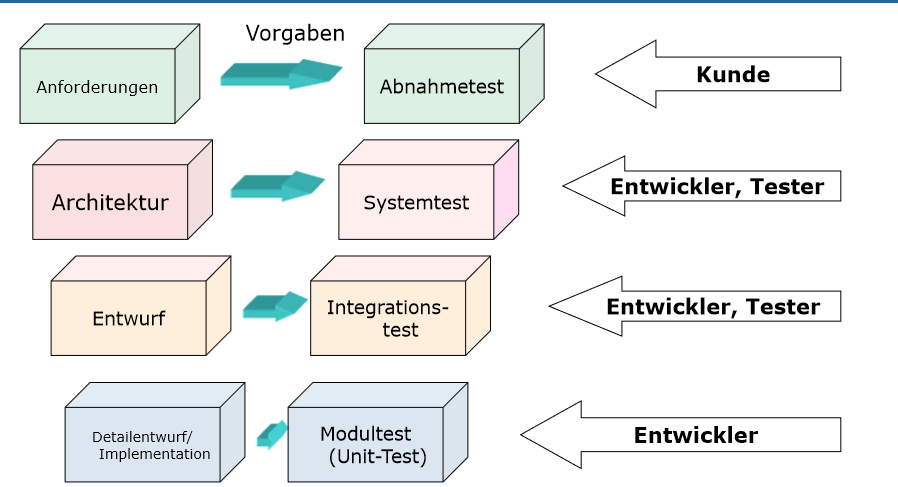
\includegraphics[width=\columnwidth]{Images/testen}
\end{center}

Dabei wird unterschieden zwischen \textbf{Verifikation}: Überprüfen ob die Vorgaben erfüllt sind (Sind alle Anforderungen im Pflichtenheft umgesetzt) und \textbf{Validierung}: Überprüfen ob Anforderungen auch ihren Nutzen erfüllen.

\subsection{Statisch vs Dynamisch Test}
Bei dynamischen Tests wird SUT (Software under Test) ausgeführt zB mittels UnitTests. Bei statische Tests muss SUT nicht aufgeführt werden zB Code-Analyse oder auch Reviews.

\subsubsection{Review}
Bei einem Review wird SUT von einem festgelegten Team auf Fehler untersucht. Fehler werden in einem Review-Bericht gesammelt und am schluss unterzeichnet. Typisches vorgehen bei einem Review:
\begin{center}
	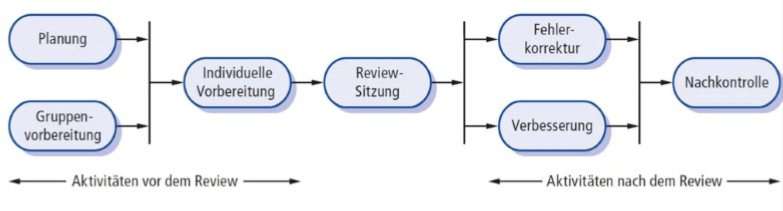
\includegraphics[width=\columnwidth]{Images/review}
\end{center}


\subsection{Black-Box Test}
Beim \textbf{Black-Box} Test gibt es keine Kenntnisse über das Innenleben. Nur Inputs und Outputs können getestet werden. 

\subsubsection{Äquivalenzklassen}
Bei diesem Verfahren werden Wertebereiche definiert, bei dem SUT das gleiche Verhalten erwartet wird. Anschliessend wird pro Klasse ein Testfall erstellt.~\\
\textbf{Beispiel} 

\begin{center}
	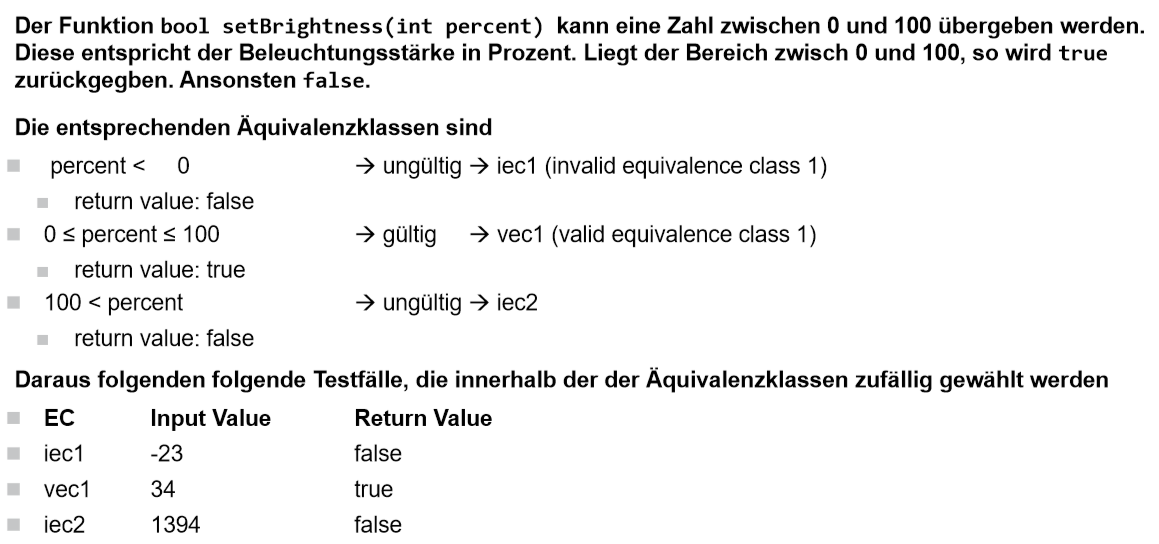
\includegraphics[width=\columnwidth]{Images/aequivalenzklassen}
\end{center}

\subsubsection{Grenzwertanalyse}
Diese Methode kann Äquivalenzklassenmethode erweitern. Die Erfahrung zeigt, dass Fehler häufig bei den Grenzen zwischen Äquivalenzklassen entstehen.
\begin{center}
	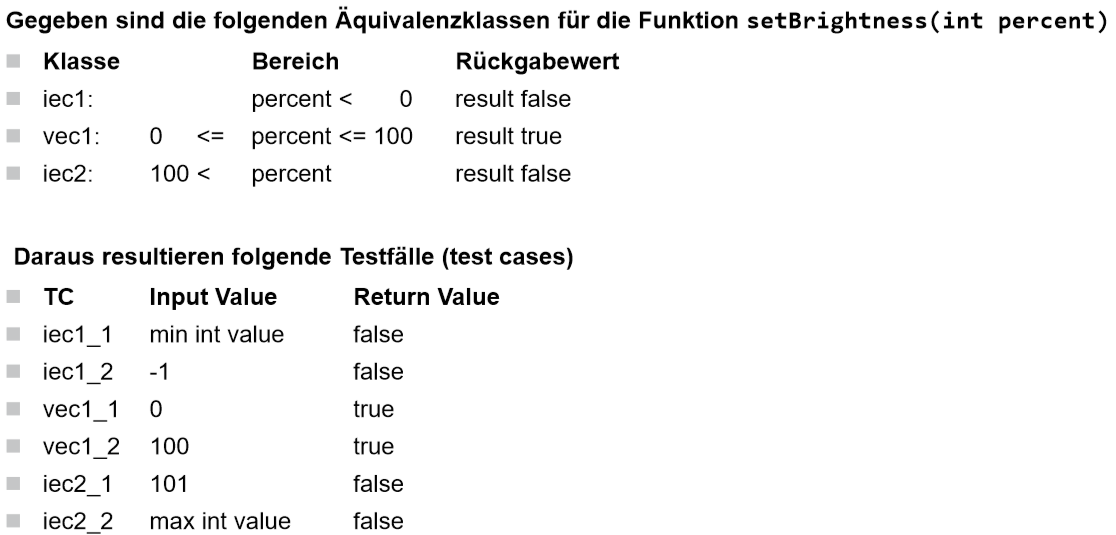
\includegraphics[width=\columnwidth]{Images/grenzwert}
\end{center}

\subsection{White-Box Test}
 Im gegensatz zur Black-Box ist das Innenleben bei \textbf{White-Test} bekannt. Dadurch ist es theoretisch möglich, alle Möglichkeiten zu testen. Dies wird in einem Code-Coverage bericht festgehalten.
 
\subsection{Testframework - googletest}
Mittels Testframework können Software Tests automatisiert werden. 
\begin{lstlisting}
TEST(KlasseName, TestMethodName) {
	MyClasse c1;
	ASSERT_EQ(c1.getValue(), 1);
}
\end{lstlisting}
Weitere Asserts:
\begin{itemize}[nosep]
	\item ASSERT\_EQ,NE,GT,GE,LT,LE(val1, val2)
	\item ASSERT\_TRUE,FALSE(condition)
	\item ASSERT\_STREQ,STRNE(str1, str2)
	\item EXPECT\_FLOAT\_EQ(val1, val2)
\end{itemize}